\documentclass{article}
\usepackage{svg}
\usepackage{graphicx}
\usepackage{hyperref}
\usepackage[T1]{fontenc}
\usepackage{listings}
\usepackage{float}
\usepackage{xcolor}
\usepackage{subcaption}
\usepackage{amsmath}
\usepackage[margin=3cm]{geometry}
\graphicspath{{../images/}{img/}}

\lstset{
    language=Python,
    basicstyle=\footnotesize\ttfamily,
    keywordstyle=\color{blue},
    commentstyle=\color{gray},
    stringstyle=\color{orange},
    breaklines=true,
    frame=lines,
    numbers=left,
    numberstyle=\tiny\color{gray}
}

\title{Vision Module - Technical Documentation}
\author{Mikołaj Baran, Kewin Kisiel, Szymon Wójcik}
\date{March 2026}

\begin{document}

\maketitle
\tableofcontents
\newpage

\section{Introduction}
The primary objective of this project is the construction of a robotic head capable of two-way communication and emotional expression. The vision system's core responsibility is detecting user faces, extracting landmarks, and identifying affective states across seven categories: anger, sadness, fear, surprise, disgust, happiness, and neutral. The output data is utilized to personalize interactions via the speech synthesis subsystem.

\section{Dataset Composition and Preprocessing}

\subsection{Data Sources}
The training corpus was aggregated from diverse repositories to ensure high variance and reliability. Key sources included:
\begin{itemize}
    \item \textbf{Public Repositories:} Aggregated versions of FER-2013, RAF-DB, and AffectNet datasets.
    \item \textbf{Synthetic Data:} Images generated using the Gemini 2.0 model and expert-annotated benchmarks.
    \item \textbf{Exp-W Dataset:} An additional 19,290 images from the "Emotion Recognition in the Wild" dataset were integrated.
    \item \textbf{Flux.1 Generation:} 10,000 high-fidelity prompts were processed using the Flux.1 [dev] model to balance ethnic diversity.
\end{itemize}

\subsection{Filtration and Cleaning Pipeline}
To eliminate informational noise, the following algorithmic filters were applied:
\begin{itemize}
    \item \textbf{Deduplication (pHash):} Perceptual hashing detected and removed 83,380 duplicated or near-duplicate images.
    \item \textbf{Demographic Filtering:} Images depicting infants (0-2 years) were removed using ViT-Age classifiers.
    \item \textbf{Artifact Removal:} EasyOCR identified and rejected samples containing text overlays.
    \item \textbf{Non-photorealistic Filtering:} The CLIP model was used to exclude caricatures and 3D renders.
\end{itemize}
After manual verification and annotation correction, the final unified dataset reached \textbf{121,133 normalized images}.

\subsection{RGB Conversion and 224px Rescaling}
While initial models utilized 96x96 grayscale images, standard DCNN architectures require 224x224 RGB inputs. To maintain consistency, a deep learning-based colorization algorithm using the CIE Lab color space was implemented.
\begin{itemize}
    \item The \textbf{L} channel (brightness) was preserved from the original grayscale for sharpness.
    \item The \textbf{a} and \textbf{b} channels (chrominance) were estimated by a DCNN to reconstruct color information.
\end{itemize}

\section{Neural Network Architectures and Training}

\subsection{Custom Models (Grayscale 96x96)}
These models served as the project baseline to establish feature extraction capabilities.

\subsubsection{first\_model}
A classical CNN optimized for spatial feature extraction.
\begin{itemize}
    \item \textbf{Accuracy:} 56.17\%.
    \item \textbf{Observation:} Experienced rapid overfitting starting at the 10th epoch.
\end{itemize}

\subsubsection{second\_model and third\_model}
Improved architectures with deeper extraction blocks and aggressive dropout rates.
\begin{itemize}
    \item \textbf{second\_model Accuracy:} 71.04\%.
    \item \textbf{third\_model Accuracy:} 67.81\%.
\end{itemize}

\subsection{ConvNeXt Tiny Implementation Details}
For both training runs of the ConvNeXt Tiny model, a consistent architectural configuration and two-phase training strategy were employed.

\subsubsection{Common Model Configuration}
The model was built using the \texttt{ConvNeXtTiny} base with \texttt{weights='imagenet'} and \texttt{include\_top=False}. The custom classification head integrated:
\begin{itemize}
    \item \textbf{GlobalAveragePooling2D:} To reduce spatial dimensions.
    \item \textbf{BatchNormalization:} For internal covariate shift stabilization.
    \item \textbf{Dropout (0.4):} To provide strong regularization.
    \item \textbf{Dense Layers:} One layer with 256 neurons (ReLU) and an output layer with 7 neurons (Softmax).
\end{itemize}

\subsubsection{Two-Phase Training Strategy}
Both runs followed a transfer learning workflow:
\begin{enumerate}
    \item \textbf{Phase 1 (Warm-up):} The base model was frozen (\texttt{trainable = False}). The classification head was trained for 5 epochs using the Adam optimizer with a learning rate of $1 \times 10^{-3}$ and \texttt{sparse\_categorical\_crossentropy} loss.
    \item \textbf{Phase 2 (Fine-Tuning):} The entire base model was unfrozen (\texttt{trainable = True}). The network was re-compiled with a significantly lower learning rate of $1 \times 10^{-5}$ to preserve ImageNet features while adapting to facial expressions.
\end{enumerate}

\subsection{ConvNeXt Tiny Training Runs Comparison}

\subsubsection{Run 1: Extended Fine-Tuning (20 Epochs Target)}
In this iteration, the fine-tuning phase was scheduled for 20 epochs with an \texttt{EarlyStopping} callback monitoring \texttt{val\_accuracy} (patience=5).
\begin{itemize}
    \item \textbf{Stability:} The process was interrupted at epoch 15 due to a kernel crash caused by hardware memory exhaustion.
    \item \textbf{Peak Metrics:} Before the crash, the model achieved its highest recorded accuracy of \textbf{74.56\%} and a macro-precision of approximately \textbf{73.55\%}.
\end{itemize}

\subsubsection{Run 2: Stable Fine-Tuning (10 Epochs Target)}
To ensure a complete training cycle and avoid further hardware failures, the second run was capped at 10 epochs for the fine-tuning phase.
\begin{itemize}
    \item \textbf{Stability:} The training finished successfully, generating a final \texttt{.keras} model file.
    \item \textbf{Final Metrics:} Achieved a validation accuracy of \textbf{73.60\%} and a macro-precision of \textbf{72.64\%}.
\end{itemize}

\subsection{Xception (with Class Balancing)}
The Xception architecture was evaluated using the same unified 121,133 image dataset, resized to 224x224 RGB. A defining characteristic of this specific model's training run was the utilization of computed class weights to counteract significant dataset imbalance across the seven emotion categories.

\subsubsection{Architecture and Configuration}
The model utilized the \texttt{Xception} base pre-trained on ImageNet (\texttt{include\_top=False}). The custom classification head was constructed as follows:
\begin{itemize}
    \item \textbf{GlobalAveragePooling2D:} To flatten spatial features.
    \item \textbf{BatchNormalization:} For internal covariate stabilization.
    \item \textbf{Dropout (0.3):} A lower dropout rate compared to the ConvNeXt run, tailored for this specific architecture.
    \item \textbf{Dense Layers:} One layer with 256 neurons (ReLU activation) and a final 7-neuron output layer (Softmax).
\end{itemize}

\subsubsection{Training Strategy}
The training process utilized computed class weights based on inverse class frequencies (loaded from \texttt{class\_weights.json}) to heavily penalize misclassifications of minority classes (like 'disgust' or 'fear'). The strategy involved two phases:

\begin{enumerate}
    \item \textbf{Phase 1 (Warm-up):} The Xception base was frozen. The classification head was trained for 10 epochs (interrupted early by callbacks after epoch 4) using the Adam optimizer with a learning rate of $1 \times 10^{-3}$ and monitoring \texttt{val\_loss}.
    \item \textbf{Phase 2 (Fine-Tuning):} The entire Xception base was unfrozen (\texttt{trainable=True}). The network was re-compiled with a significantly lower learning rate of $1 \times 10^{-4}$. Training was scheduled for an additional 20 epochs starting from epoch 4, but finished early after epoch 11 due to early stopping criteria.
\end{enumerate}

\subsubsection{Results and Performance}
The Xception model achieved a final validation accuracy of \textbf{64.92\%}. The confusion matrix reveals high accuracy for 'happiness' and 'neutral' expressions, but significant challenges in differentiating 'fear' and 'disgust', which were frequently misclassified as 'sadness' or 'anger', despite the application of class weights.

\begin{figure}[H]
    \centering
    \begin{minipage}{0.48\textwidth}
        \centering
    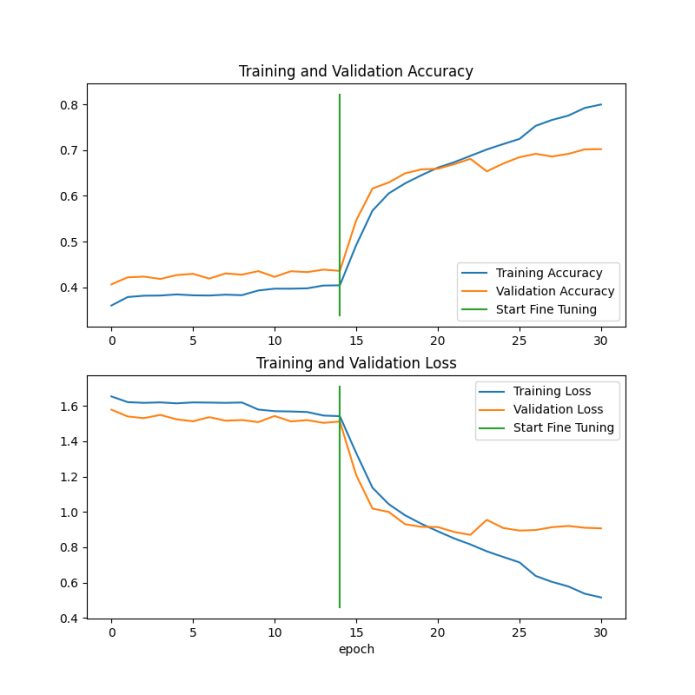
\includegraphics[width=\linewidth]{xception_history.png}
        \caption{Training history: Xception Accuracy and Loss}
        \label{fig:xception_history}
    \end{minipage}\hfill
    \begin{minipage}{0.48\textwidth}
        \centering
        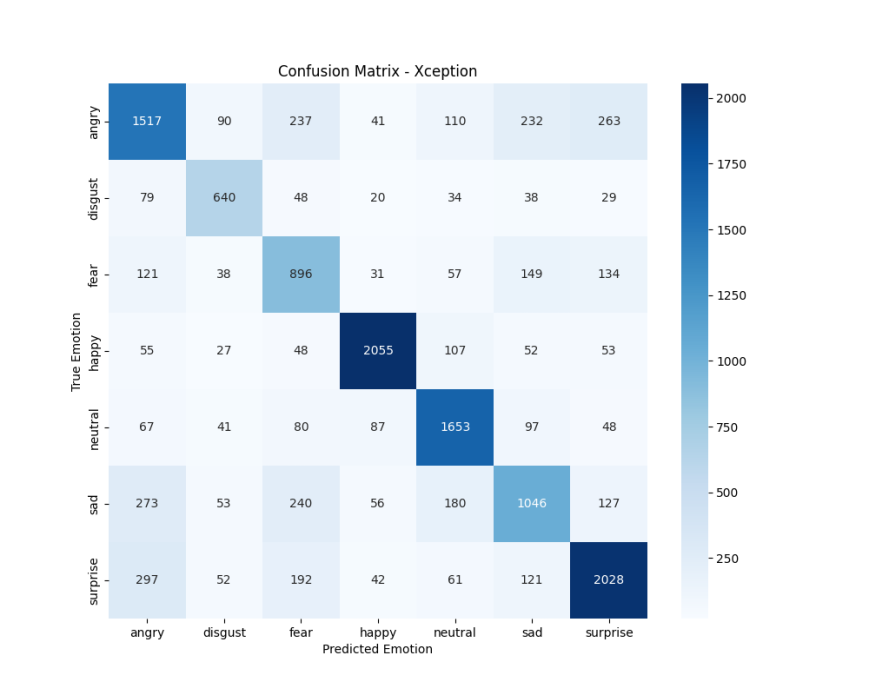
\includegraphics[width=\linewidth]{xception_cm.png}
        \caption{Normalized Confusion Matrix: Xception}
        \label{fig:xception_cm}
    \end{minipage}
\end{figure}

\subsection{ResNet50 (Initial Training Run)}
The ResNet50 architecture was evaluated using the standardized 224x224 RGB dataset. This section details the initial training iteration before further optimizations.

\subsubsection{Architecture and Configuration}
The model utilized the \texttt{ResNet50} base pre-trained on ImageNet (\texttt{include\_top=False}). The custom classification head was constructed with:
\begin{itemize}
    \item \textbf{GlobalAveragePooling2D:} To reduce spatial dimensions.
    \item \textbf{BatchNormalization:} For stabilizing the learning process.
    \item \textbf{Dropout (0.4):} Applied as a strong regularization measure.
    \item \textbf{Dense Layers:} One fully connected layer with 256 neurons (ReLU) and a final 7-neuron output layer (Softmax).
\end{itemize}

\subsubsection{Training Strategy}
The initial training run followed a standard two-phase transfer learning approach without explicit class weights:
\begin{enumerate}
    \item \textbf{Phase 1 (Warm-up):} The base model was frozen. The classification head was trained for 5 epochs using the Adam optimizer ($LR = 1 \times 10^{-3}$).
    \item \textbf{Phase 2 (Fine-Tuning):} The entire base model was unfrozen, and the learning rate was reduced to $1 \times 10^{-5}$. The training was scheduled for 15 epochs with an \texttt{EarlyStopping} callback monitoring validation accuracy (patience of 5).
\end{enumerate}

\subsubsection{Results and Performance}
In this first training run, the ResNet50 model achieved a validation accuracy of \textbf{67.89\%} and a macro-precision of \textbf{66.21\%}.

\begin{figure}[H]
    \centering
    \begin{minipage}{0.48\textwidth}
        \centering
        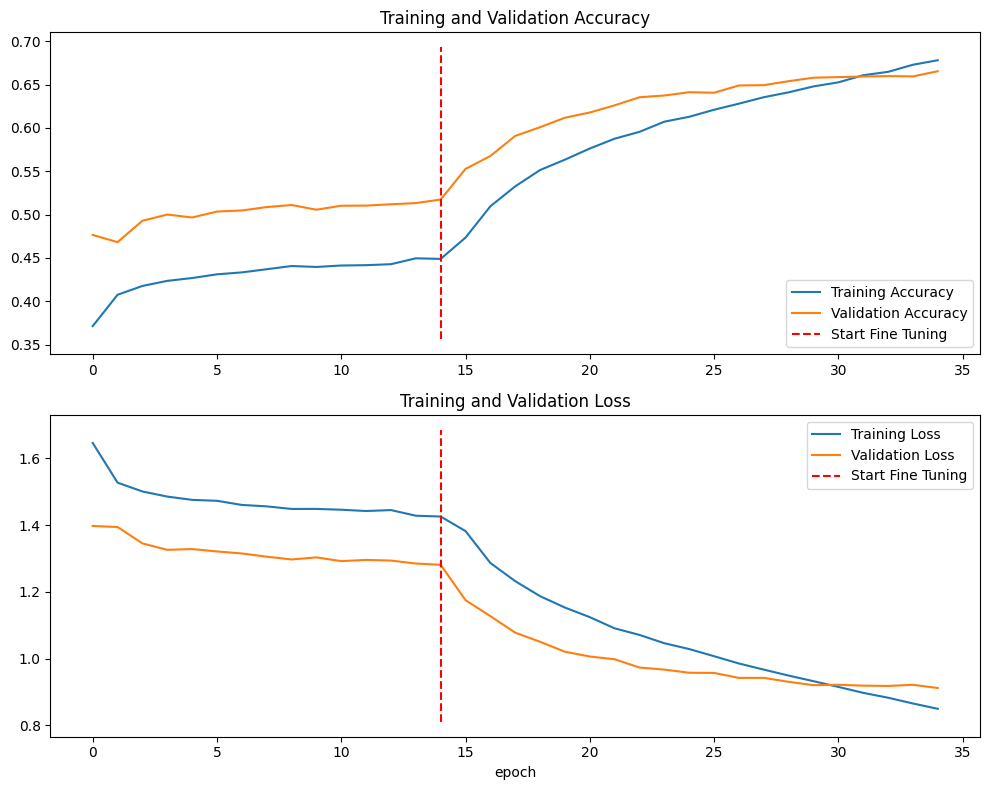
\includegraphics[width=\linewidth]{resnet50_run1_history.png}
        \caption{Training history: ResNet50 (Run 1)}
        \label{fig:resnet50_run1_history}
    \end{minipage}\hfill
    \begin{minipage}{0.48\textwidth}
        \centering
        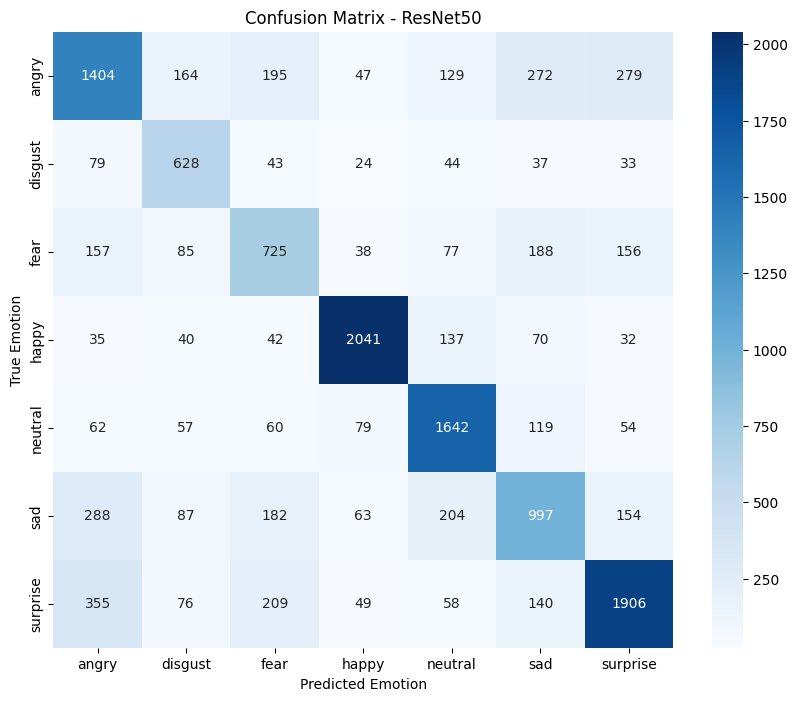
\includegraphics[width=\linewidth]{resnet50_run1_cm.png}
        \caption{Confusion Matrix: ResNet50 (Run 1)}
        \label{fig:resnet50_run1_cm}
    \end{minipage}
\end{figure}

\subsection{ResNet50 - Second Training Run}
To surpass the performance of previous iterations, a second training run for the ResNet50 model was conducted using a refined two-stage transfer learning strategy. The model architecture was extended with a custom classification head: Global Average Pooling, Batch Normalization, a Dropout layer (0.4), and a Dense layer with 256 units using ReLU activation.

The training parameters and process were structured as follows:
\begin{itemize}
    \item \textbf{Phase 1 (Warm-up):} 5 epochs with a frozen ResNet50 base, utilizing the Adam optimizer with a learning rate of $1 \times 10^{-3}$.
    \item \textbf{Phase 2 (Fine-tuning):} The base was unfrozen and trained for 10 epochs with a significantly lower learning rate of $1 \times 10^{-5}$ to perform subtle weight adjustments.
    \item \textbf{Callbacks:} \texttt{EarlyStopping} was implemented with a patience of 5 and, crucially, \texttt{restore\_best\_weights=True}.
\end{itemize}

\begin{figure}[H]
    \centering
    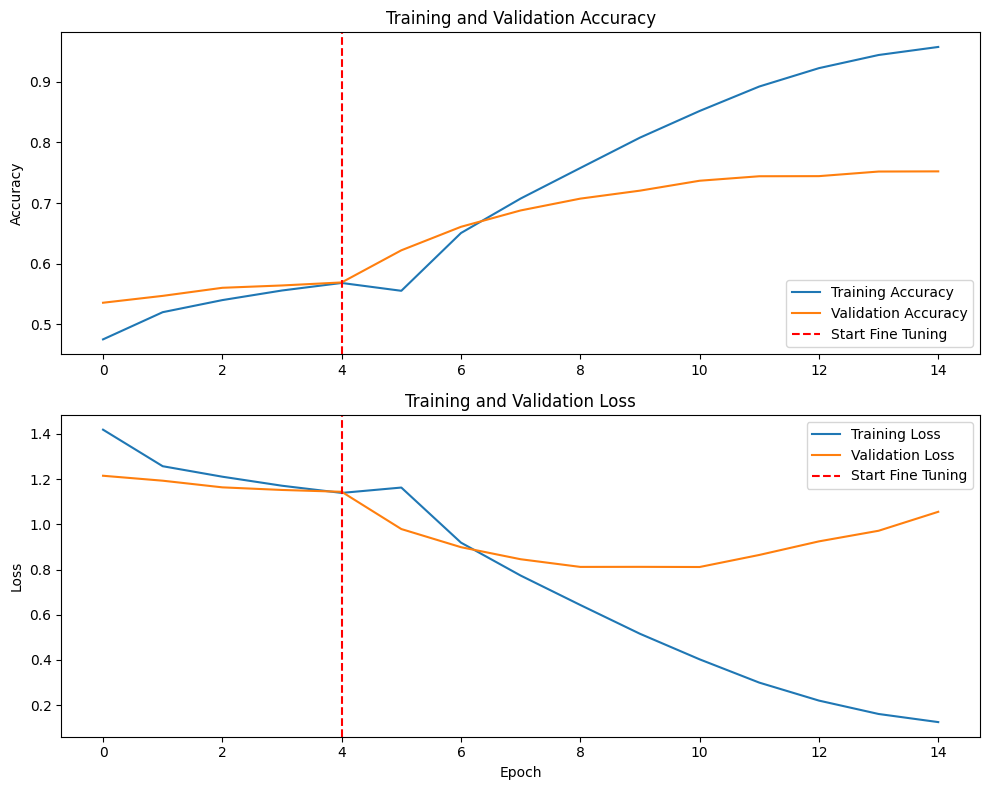
\includegraphics[width=0.8\textwidth]{resnet50_run2_history.png}
    \caption{Training and validation metrics for the ResNet50 second run. The dashed red line indicates the transition from warm-up to fine-tuning.}
    \label{fig:resnet50_history}
\end{figure}

The learning curves (Fig. \ref{fig:resnet50_history}) show a successful convergence. A notable observation is the behavior during the final epochs of fine-tuning: while the training loss continued to decrease, the validation loss showed a slight upward trend, indicating the onset of overfitting. However, due to the \texttt{restore\_best\_weights} parameter, the training process effectively "rewound" the model to the state of epoch 11, where validation accuracy was maximized and loss was at its lowest.

\begin{figure}[H]
    \centering
    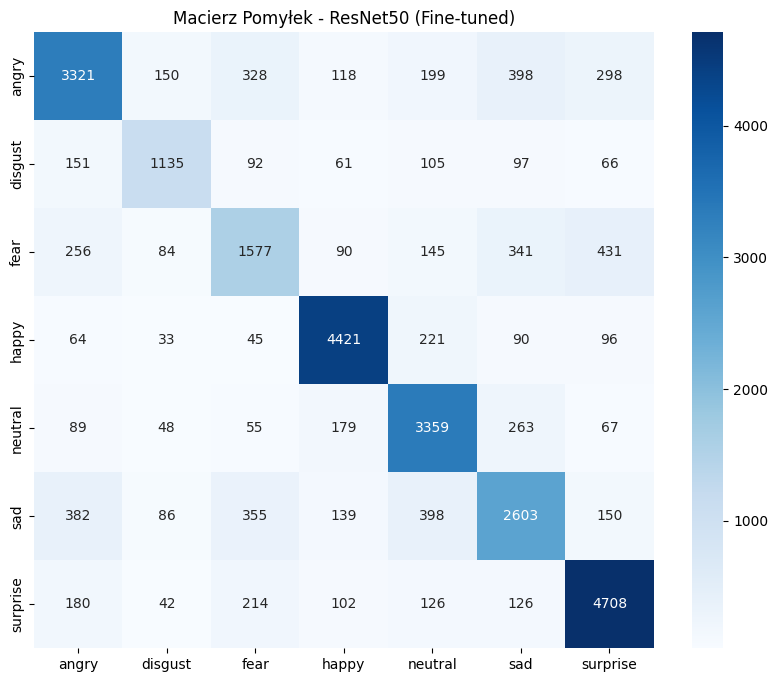
\includegraphics[width=0.7\textwidth]{resnet50_run2_cm.png}
    \caption{Confusion matrix for the optimized ResNet50 model.}
    \label{fig:resnet50_cm}
\end{figure}

The final model achieved a peak accuracy of \textbf{75.22\%} and a macro-precision of \textbf{73.36\%}. As shown in the confusion matrix (Fig. \ref{fig:resnet50_cm}), the model excels at identifying \textit{happy} and \textit{neutral} expressions. Consistent with previous models, the primary confusion occurs between \textit{sad} and \textit{neutral} classes, which is expected given the visual similarity of these expressions in the dataset. This result represents the best performance achieved in the project thus far.

\subsection{ResNet101 (Initial Training Run)}
To investigate whether a deeper residual architecture would yield better feature extraction, the \texttt{ResNet101} model was subjected to a similar initial training process.

\subsubsection{Architecture and Configuration}
The architecture closely mirrored the ResNet50 setup, utilizing the \texttt{ResNet101} base (\texttt{include\_top=False}), but with a slightly more aggressive regularization applied to the classification head:
\begin{itemize}
    \item \textbf{GlobalAveragePooling2D} and \textbf{BatchNormalization}.
    \item \textbf{Dropout (0.5):} Increased to 0.5 to counteract the higher risk of overfitting associated with a significantly deeper network.
    \item \textbf{Dense Layers:} 256 neurons (ReLU) and 7 neurons (Softmax).
\end{itemize}

\subsubsection{Training Strategy}
The two-phase training strategy was identical to the ResNet50 initial run:
\begin{enumerate}
    \item \textbf{Phase 1 (Warm-up):} Base frozen, 5 epochs, Adam optimizer ($LR = 1 \times 10^{-3}$).
    \item \textbf{Phase 2 (Fine-Tuning):} Base unfrozen, 15 epochs, Adam optimizer ($LR = 1 \times 10^{-5}$).
\end{enumerate}

\subsubsection{Results and Performance}
The initial fine-tuning of ResNet101 resulted in a validation accuracy of \textbf{67.45\%} and a macro-precision of \textbf{65.88\%}. Notably, despite its increased depth and parameter count, this initial run did not outperform the shallower ResNet50 model, indicating that the extra layers may not provide an immediate advantage for this specific dataset without further tuning.

\begin{figure}[H]
    \centering
    \begin{minipage}{0.48\textwidth}
        \centering
        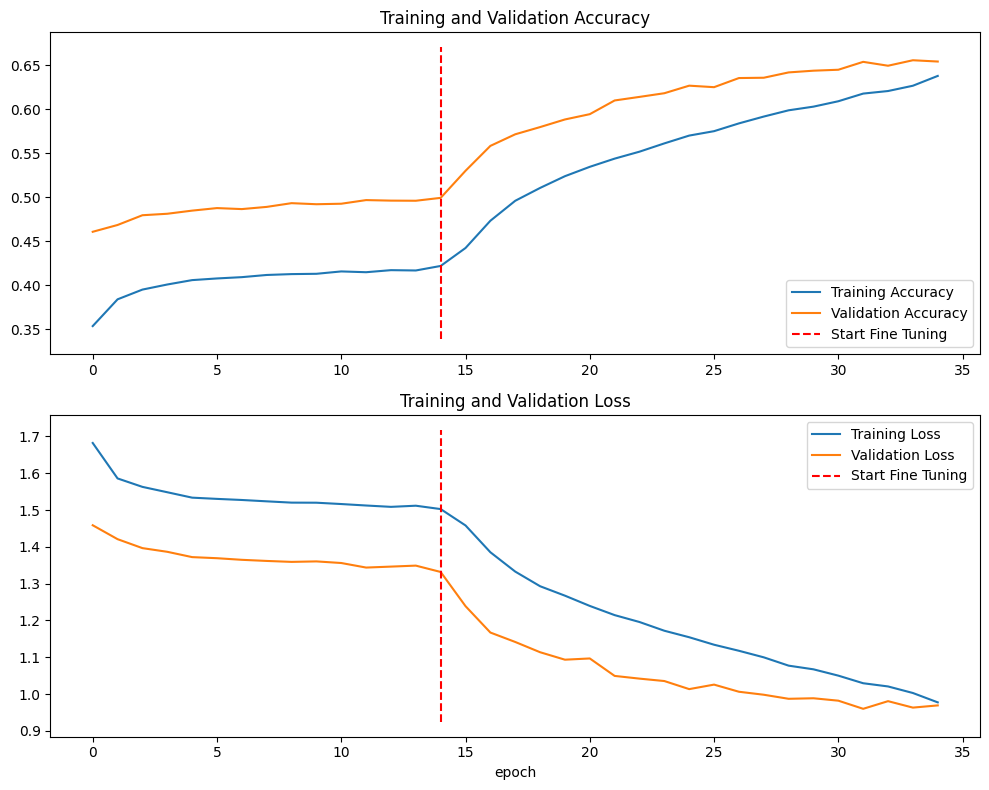
\includegraphics[width=\linewidth]{resnet101_run1_history.png}
        \caption{Training history: ResNet101 (Run 1)}
        \label{fig:resnet101_run1_history}
    \end{minipage}\hfill
    \begin{minipage}{0.48\textwidth}
        \centering
        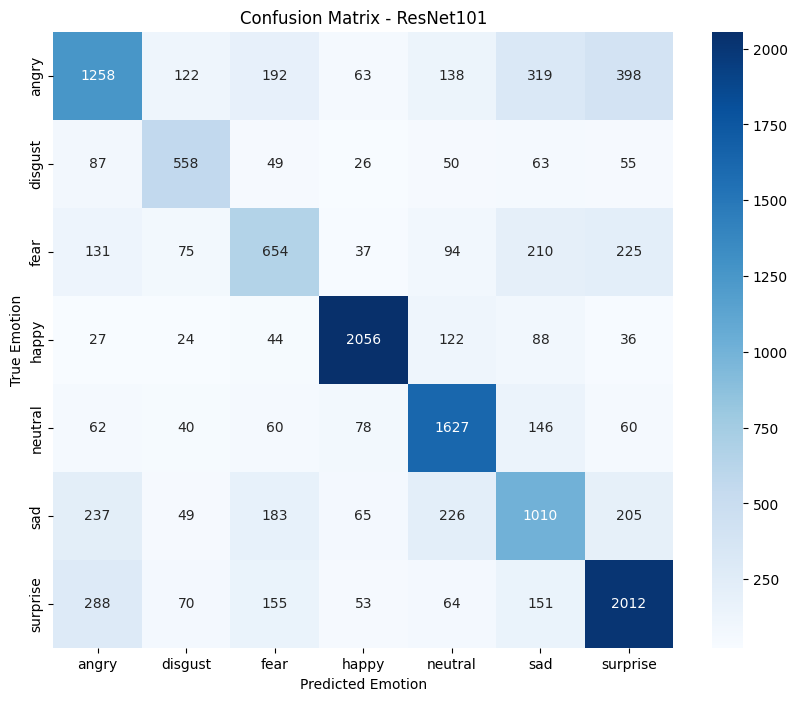
\includegraphics[width=\linewidth]{resnet101_run1_cm.png}
        \caption{Confusion Matrix: ResNet101 (Run 1)}
        \label{fig:resnet101_run1_cm}
    \end{minipage}
\end{figure}

\subsection{ResNet101 - Second Training Run}
Building upon the successful two-stage training strategy implemented for ResNet50, a parallel optimization was conducted for the deeper ResNet101 architecture. To accommodate the increased memory requirements (VRAM) of the 101-layer network, the batch size was reduced from 32 to 16. The custom classification head remained identical to the ResNet50 configuration to ensure an objective comparison.

The training process utilized the proven sequential approach:
\begin{itemize}
    \item \textbf{Phase 1 (Warm-up):} 5 epochs with a frozen base, using the Adam optimizer ($1 \times 10^{-3}$).
    \item \textbf{Phase 2 (Fine-tuning):} The entire network was unfrozen and trained for 10 epochs applying a heavily reduced learning rate ($1 \times 10^{-5}$).
    \item \textbf{Callbacks:} \texttt{EarlyStopping} configured with \texttt{restore\_best\_weights=True} (patience=5) and \texttt{ModelCheckpoint} to secure optimal weights.
\end{itemize}

\begin{figure}[H]
    \centering
    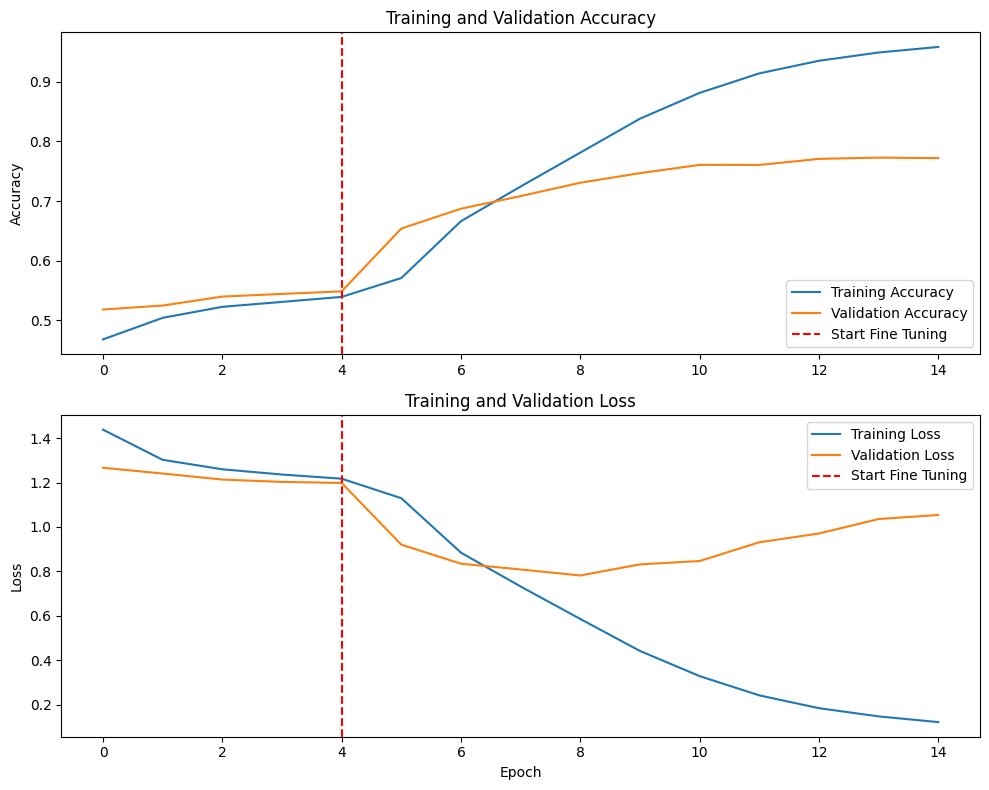
\includegraphics[width=0.8\textwidth]{resnet101_run2_history.png}
    \caption{Training and validation metrics for the ResNet101 second run. The deeper architecture benefits significantly from the two-stage fine-tuning approach.}
    \label{fig:resnet101_history}
\end{figure}

The learning curves (Fig. \ref{fig:resnet101_history}) demonstrate a highly effective training cycle. The transition into fine-tuning initially yields steady improvements in both metrics. As the training progresses, a divergence between the training and validation loss emerges, signaling the onset of overfitting as the high-capacity model begins memorizing the training set. Fortunately, the \texttt{EarlyStopping} mechanism successfully intervened, rewinding the weights to the exact epoch where validation accuracy peaked.

\begin{figure}[H]
    \centering
    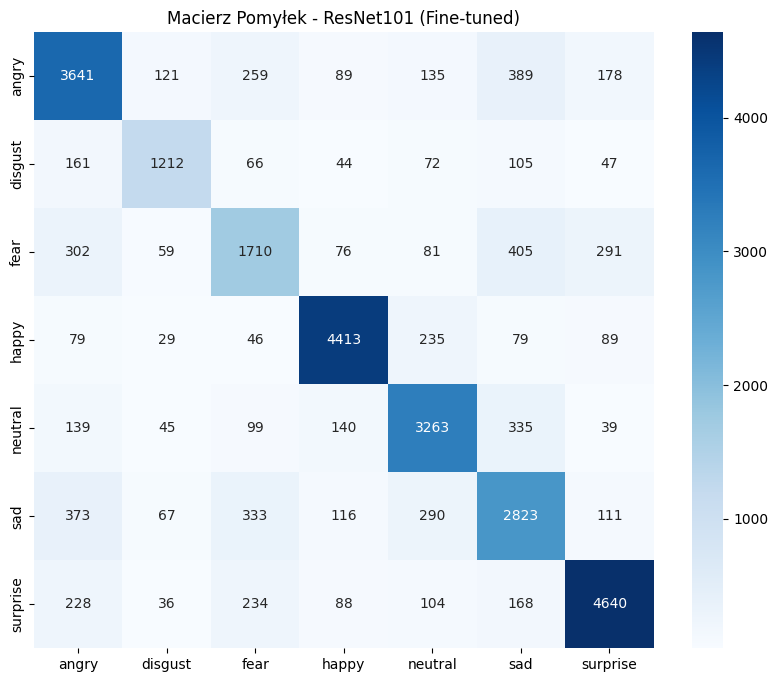
\includegraphics[width=0.7\textwidth]{resnet101_run2_cm.png}
    \caption{Confusion matrix for the optimized ResNet101 model, showing the highest overall performance.}
    \label{fig:resnet101_cm}
\end{figure}

The optimized ResNet101 achieved an outstanding final accuracy of \textbf{77.28\%} and a macro-precision of \textbf{76.00\%}, establishing it as the absolute top-performing model in the entire study. The confusion matrix (Fig. \ref{fig:resnet101_cm}) reveals robust classification across the board. While inherent dataset challenges remain (such as distinguishing between \textit{sad} and \textit{neutral}), the extra depth of ResNet101 allowed for more nuanced feature extraction, comfortably exceeding the project's baseline target of 75\%.
\subsection{ConvNextV2 - compare}
We also compared the ConvNeXt V2 model variants: Atto (3.7M parameters), Pico (9.1M parameters), Tiny (28.6M parameters), Base (89M parameters), and Huge (660M parameters). The evaluations were conducted on an NVIDIA RTX 6000 Ada Generation GPU with 48GB of VRAM. The input images were provided in RGB format at a resolution of 224x224 pixels.
\subsubsection{Architecture adn configuration}
\begin{itemize}
    \item \textbf{GlobalAveragePooling2D} and \textbf{LayerNormalization}.
    \item \textbf{Dropout (0.4):} Set to 0.4 to counteract the risk of overfitting associated with a significantly deeper network.
    \item \textbf{Dense Layers:} 256 neurons (GELU) and 7 neurons (Softmax).
\end{itemize}
\subsubsection{Pre-training}
Class weights were calculated for the dataset to mitigate the issue of an uneven number of images for individual emotions. During this phase, the entire base architecture of the ConvNeXt model was frozen, and only the newly added classification layers were trained. The learning rate was set to a constant value of 1e-3.
\subsubsection{Fine-tuning}
In this phase, the base model was unfrozen; however, to preserve the previously learned low-level image features, its initial layers ("stem", "patch", and the first two convolutional blocks) were refrozen. Only the deeper layers of the base model and the classifier were subjected to training. A variable learning rate was applied using the Cosine Decay with Restarts schedule (with an initial value of 1e-5).
\subsubsection{Results}
\begin{itemize}
    \item \textbf{ConvNeXtV2 Huge:} Macro Precision: 0.6236, Validation Accuracy: $\approx$0.656
    \item \textbf{ConvNeXtV2 Base:} Macro Precision: 0.5969, Validation Accuracy: $\approx$0.630
    \item \textbf{ConvNeXtV2 Tiny:} Macro Precision: 0.5635, Validation Accuracy: $\approx$0.597
    \item \textbf{ConvNeXtV2 Atto:} Macro Precision: 0.4841, Validation Accuracy: $\approx$0.517
    \item \textbf{ConvNeXtV2 Pico:} Macro Precision: 0.4197, Validation Accuracy: $\approx$0.405
\end{itemize}
\begin{figure}[H]
    \centering
    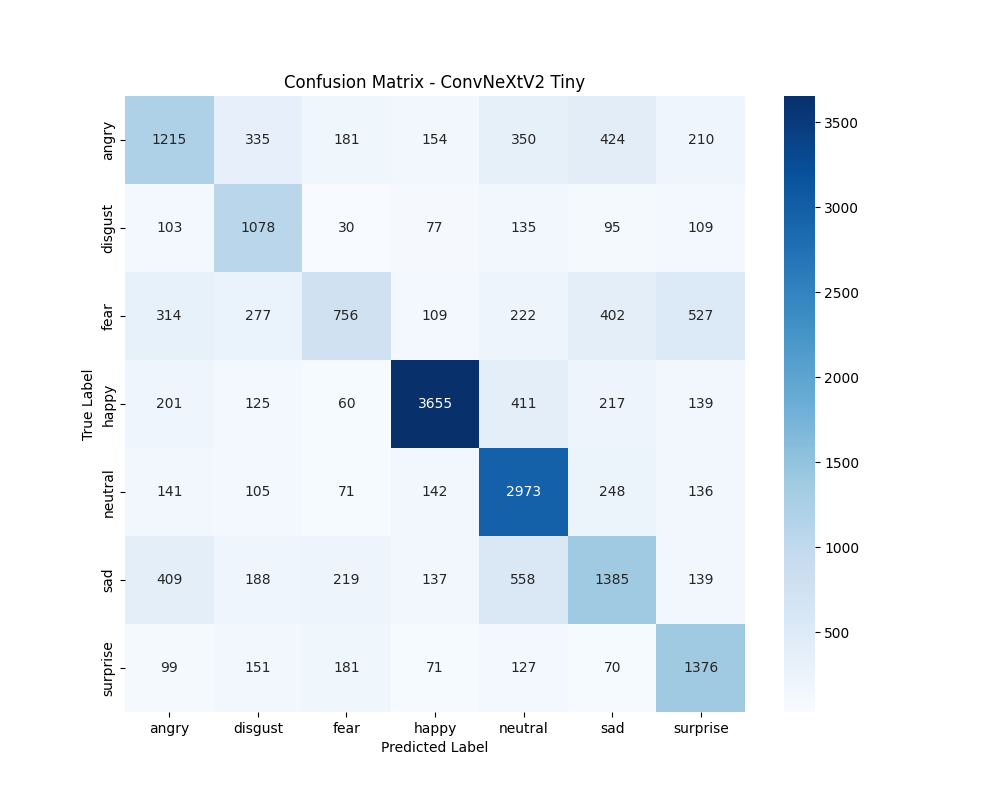
\includegraphics[width=0.7\textwidth]{TinyV2_CM.png}
    \caption{Confusion matrix for the optimized ConvNextV2 Tiny model, showing the highest overall performance.}
    \label{fig:tinyv2_cm}
\end{figure}
\begin{figure}[H]
    \centering
    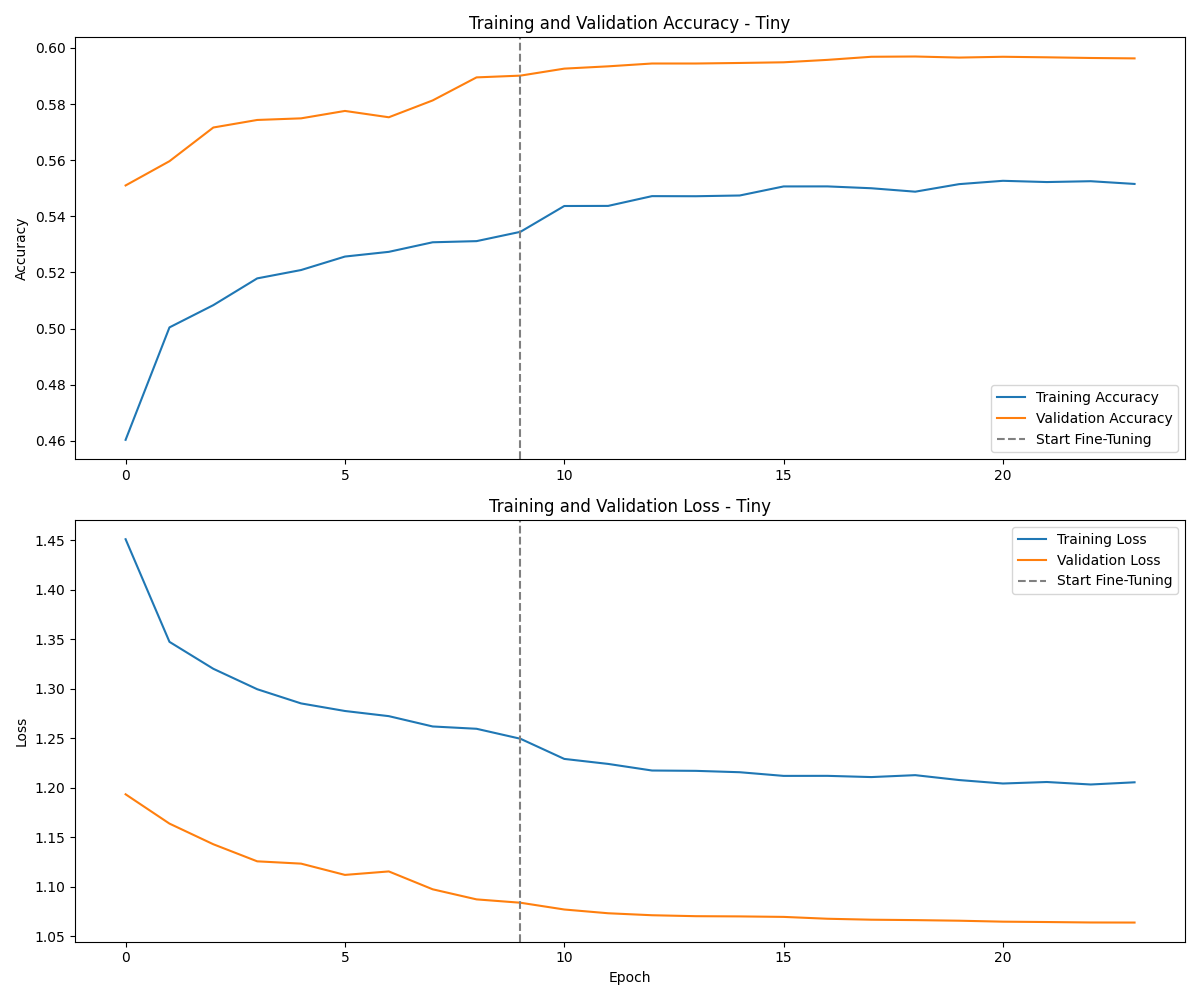
\includegraphics[width=0.7\textwidth]{TinyV2_Loss.png}
    \caption{Training and validation metrics for the ConvNextV2 Tiny second run.}
    \label{fig:tinyv2_loss}
\end{figure}

\section{ConvNeXtV2 - Custom Dataset}
We decided to compare the ConvNeXt V1 and V2 architectures. We chose five model sizes for this evaluation: Atto (3.7M parameters), Pico (9.1M parameters), Tiny (28.6M parameters), Base (89M parameters), and Huge (660M parameters).

\subsubsection{New Dataset} 
For this training, we compiled a custom dataset. It includes:
\begin{itemize}
    \item 10,000 images generated with FLUX using prompts based on the scientific definition of each emotion.
    \item 10,000 generated images that do not conform to these scientific definitions (e.g., featuring slightly turned faces). 
    \item 59,000 pictures of real humans sourced from the ExpW dataset and Viktor Modroczký's dataset (found on Kaggle; please refer to the technical documentation for details).
\end{itemize} 

We decided to create a new dataset using generated images to improve model accuracy. Upon inspecting the original dataset, we discovered it contained numerous low-quality images (e.g., poorly visible or obscured faces).

\subsubsection{Architecture and Configuration}
\begin{itemize}
    \item Augmentation includes Random Flip, 15\% rotation, 15\% zoom-in, translations, as well as brightness and contrast adjustments.
    \item We normalized the pixel values to [-1, 1], which is necessary for ConvNeXtV2 models.
    \item ConvNeXtV2 models were initialized with ImageNet weights (for the Atto and Pico variants) and ImageNet-21k-ft1k weights (for the Tiny, Base, and Huge variants).
    \item Model Architecture:
    \begin{itemize}
        \item GlobalAveragePooling2D
        \item BatchNormalization
        \item Dense (512 neurons): With GELU activation function.
        \item Dropout (0.4)
        \item Dense (256 neurons): With GELU activation function.
        \item Dropout (0.2)
        \item Output Layer (Dense): 7 neurons with Softmax activation function for emotion classification.
    \end{itemize}
\end{itemize}

\subsubsection{Pre-training}
In the first phase, we focus on training the newly added classification layers, while the previously trained base layers remain frozen.
\begin{itemize}
    \item All base layers frozen.
    \item Epochs: 10
    \item Learning Rate: Training begins with a 2-epoch warmup, after which the learning rate reaches a maximum value of 0.001, and then gradually decreases following a cosine decay schedule.
    \item Loss Function: Categorical Crossentropy.
    \item Class balancing was applied to compensate for the uneven number of samples across individual emotions.
\end{itemize}

\subsubsection{Fine-tuning}
Fine-tuning consists of two phases where we progressively unfreeze specific layers.

\paragraph{Phase 1: Partial Fine-Tuning}
\begin{itemize}
    \item The last two deepest sections of the base model, responsible for analyzing high-level semantic image features, were unfrozen. The initial layers remained frozen.
    \item Epochs: 10
    \item The base Learning Rate was reduced to 0.00003 (3e-5).
\end{itemize}

\paragraph{Phase 2: Full Fine-Tuning}
\begin{itemize}
    \item All four main sections of the base model were unfrozen.
    \item The "stem" and "patch" layers were kept frozen, as they are responsible for basic shape and edge detection.
    \item Epochs: 15
    \item A low base Learning Rate of 0.00001 (1e-5) was applied.
\end{itemize}

\subsubsection{Results}

\begin{figure}[H]
    \centering
    \begin{subfigure}[b]{0.48\textwidth}
        \centering
        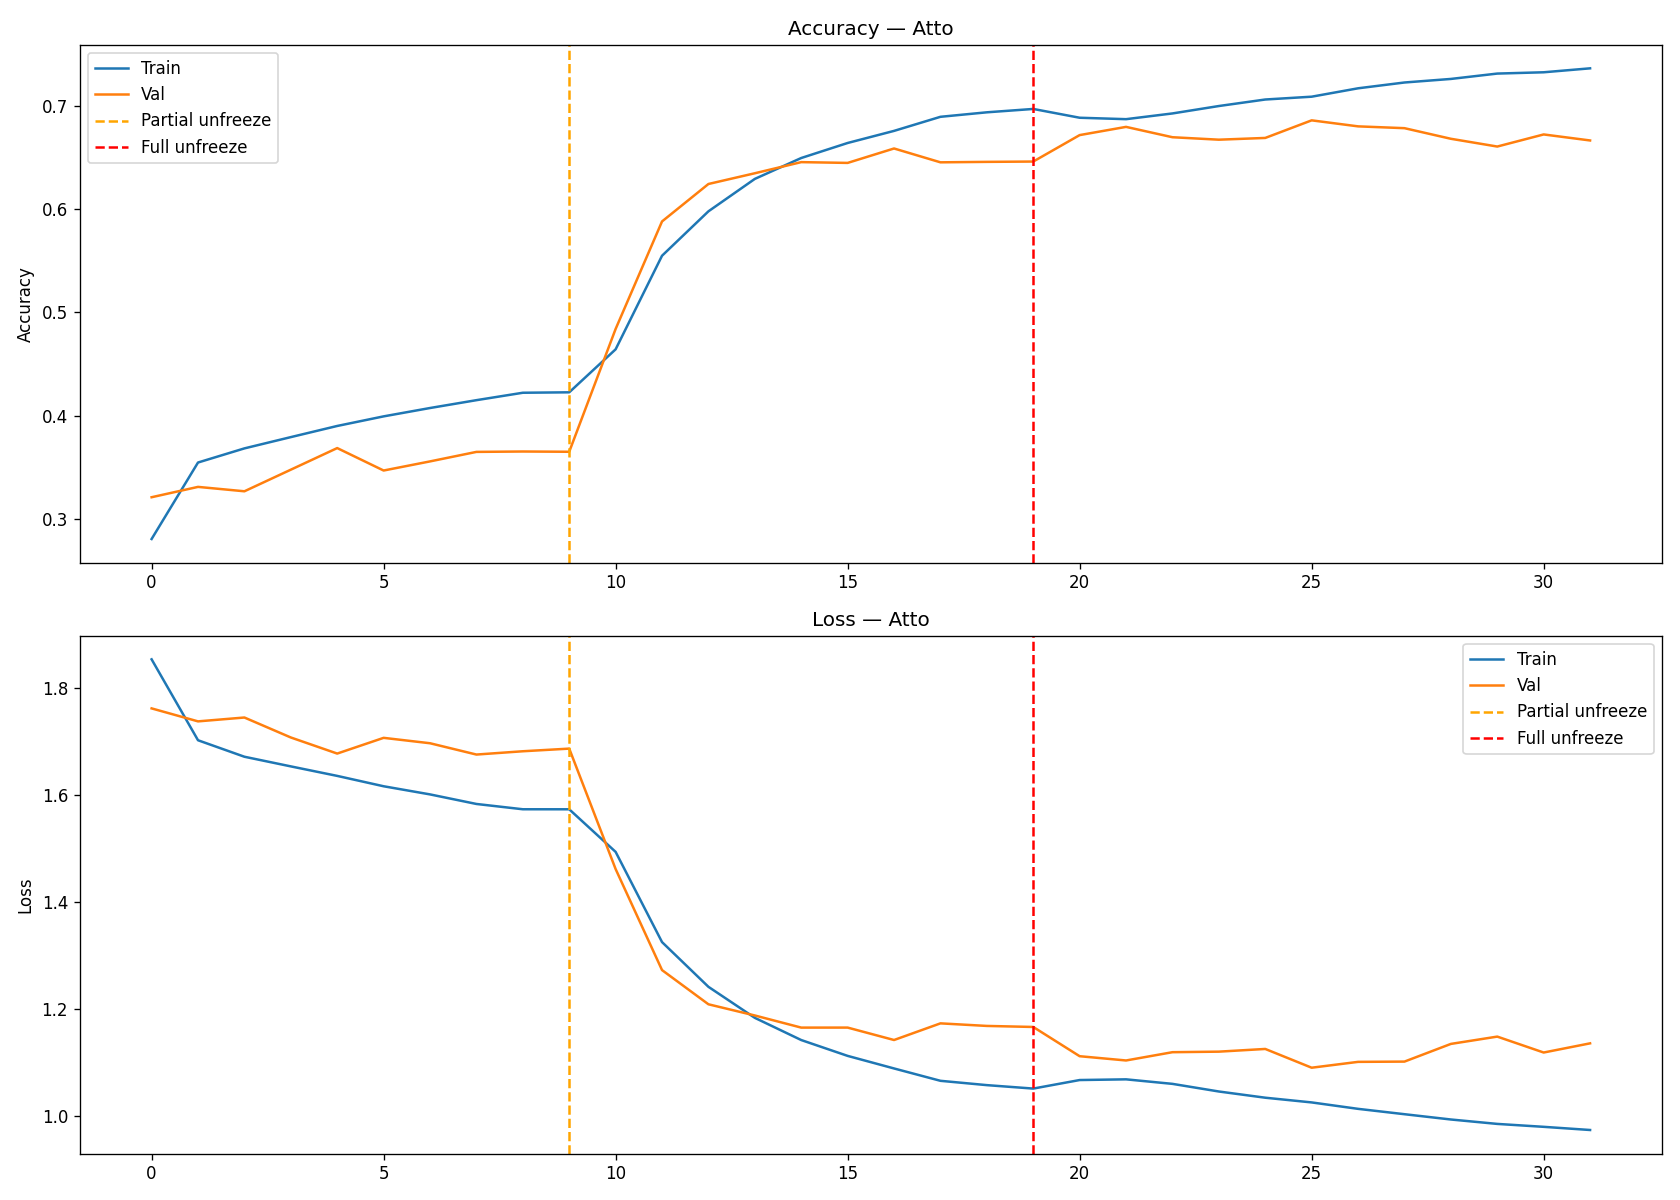
\includegraphics[width=\textwidth]{Atto_history.png}
        \caption{Atto - Training History}
        \label{fig:atto_hist}
    \end{subfigure}
    \hfill
    \begin{subfigure}[b]{0.48\textwidth}
        \centering
        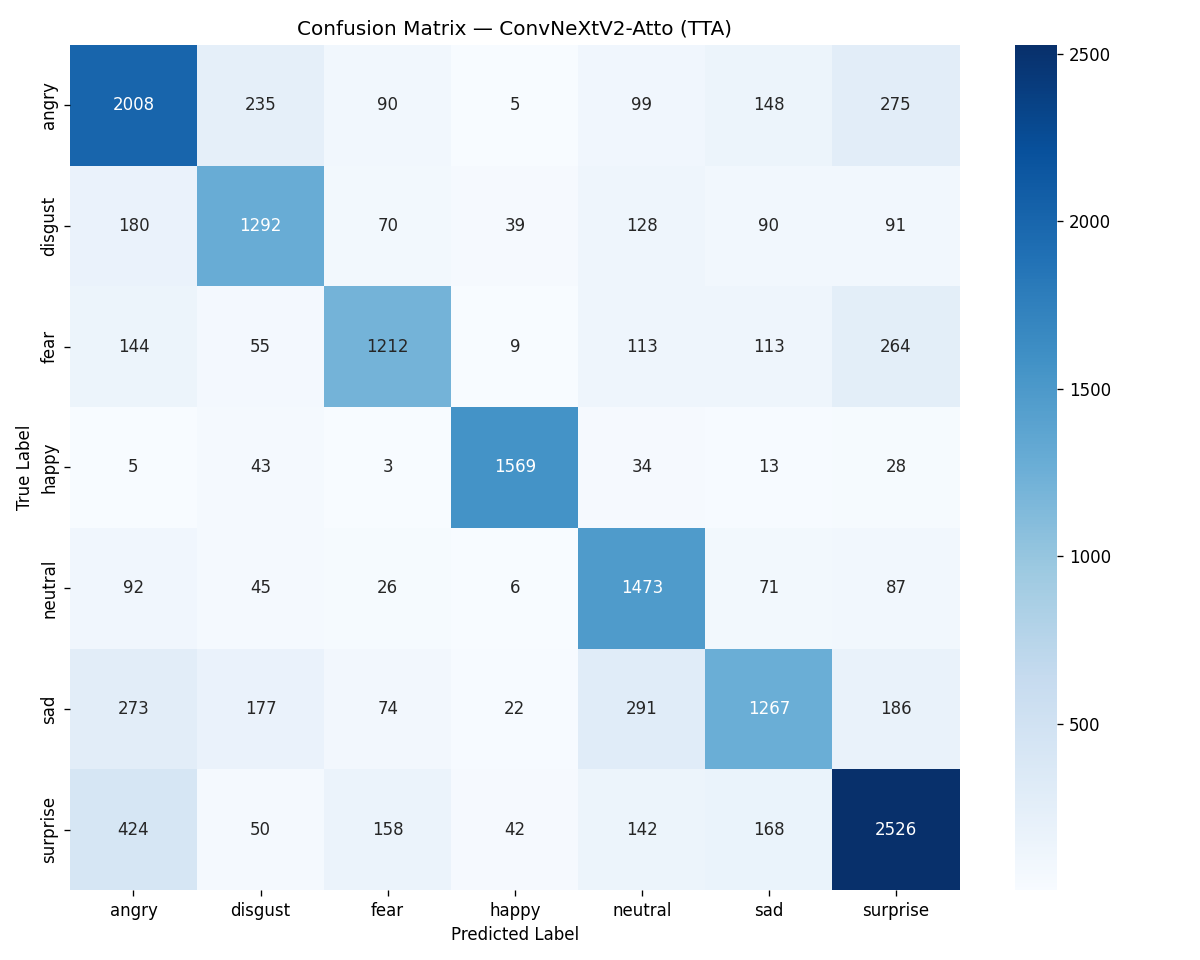
\includegraphics[width=\textwidth]{Atto_cm.png}
        \caption{Atto - Confusion Matrix}
        \label{fig:atto_cm}
    \end{subfigure}
    \vspace{1em}
    \begin{subfigure}[b]{0.48\textwidth}
        \centering
        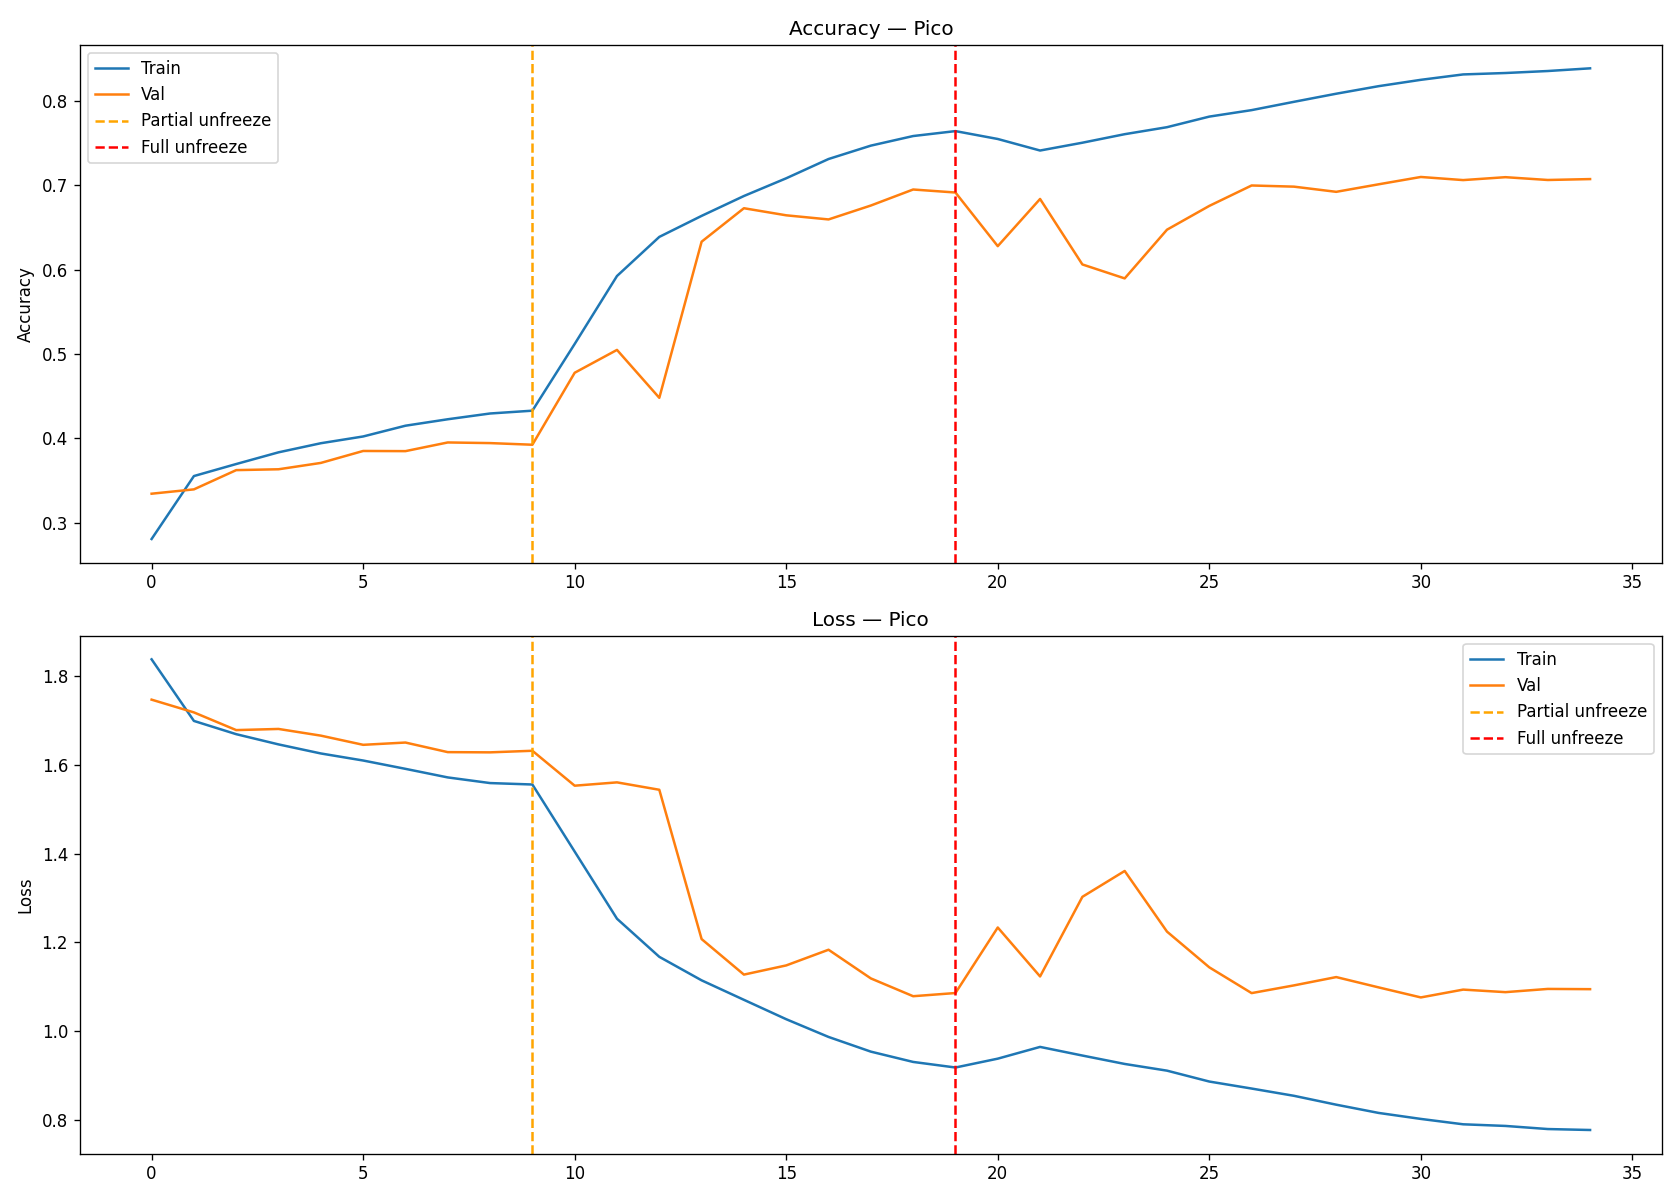
\includegraphics[width=\textwidth]{Pico_history.png}
        \caption{Pico - Training History}
        \label{fig:pico_hist}
    \end{subfigure}
    \hfill
    \begin{subfigure}[b]{0.48\textwidth}
        \centering
        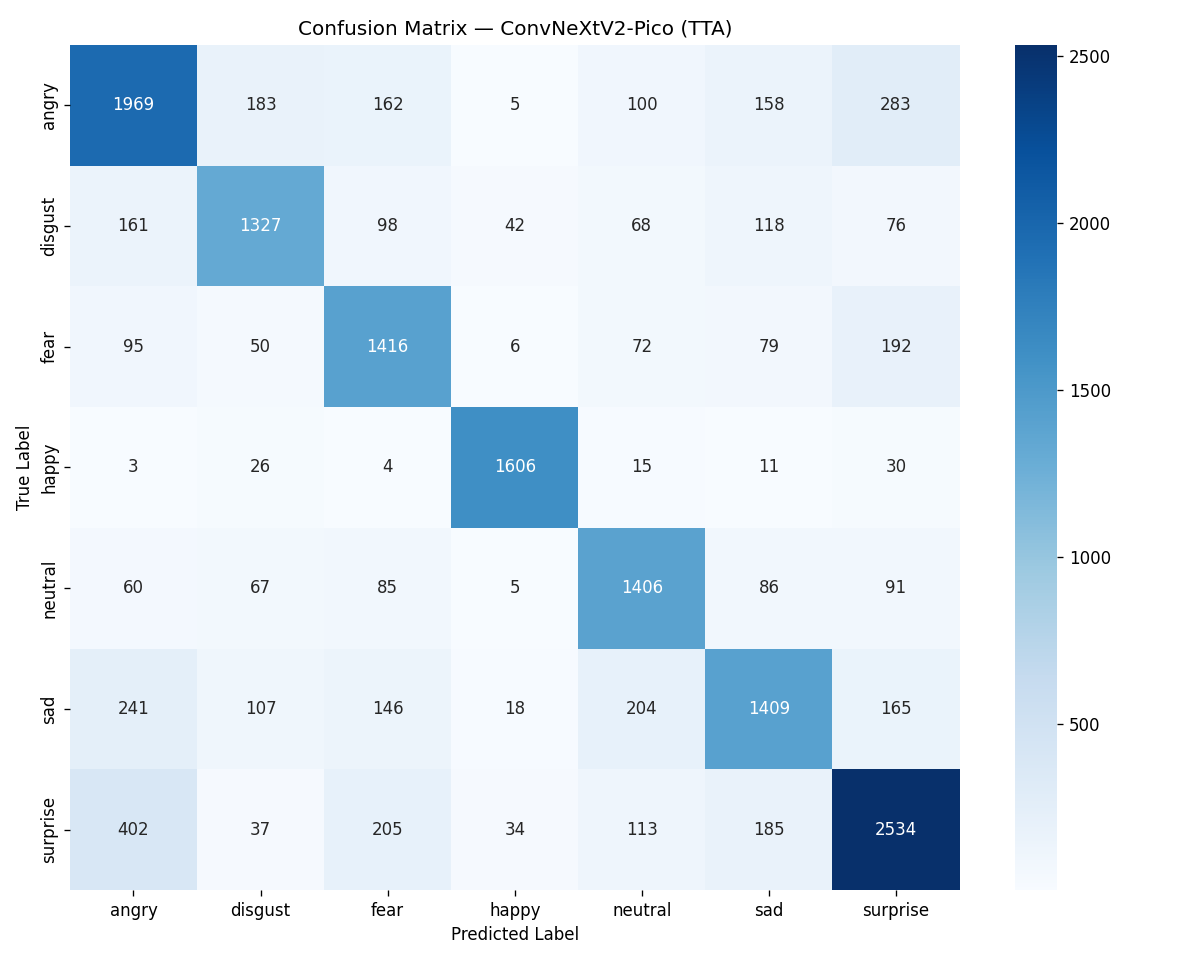
\includegraphics[width=\textwidth]{Pico_cm.png}
        \caption{Pico - Confusion Matrix}
        \label{fig:pico_cm}
    \end{subfigure}
    \vspace{1em}
    \begin{subfigure}[b]{0.48\textwidth}
        \centering
        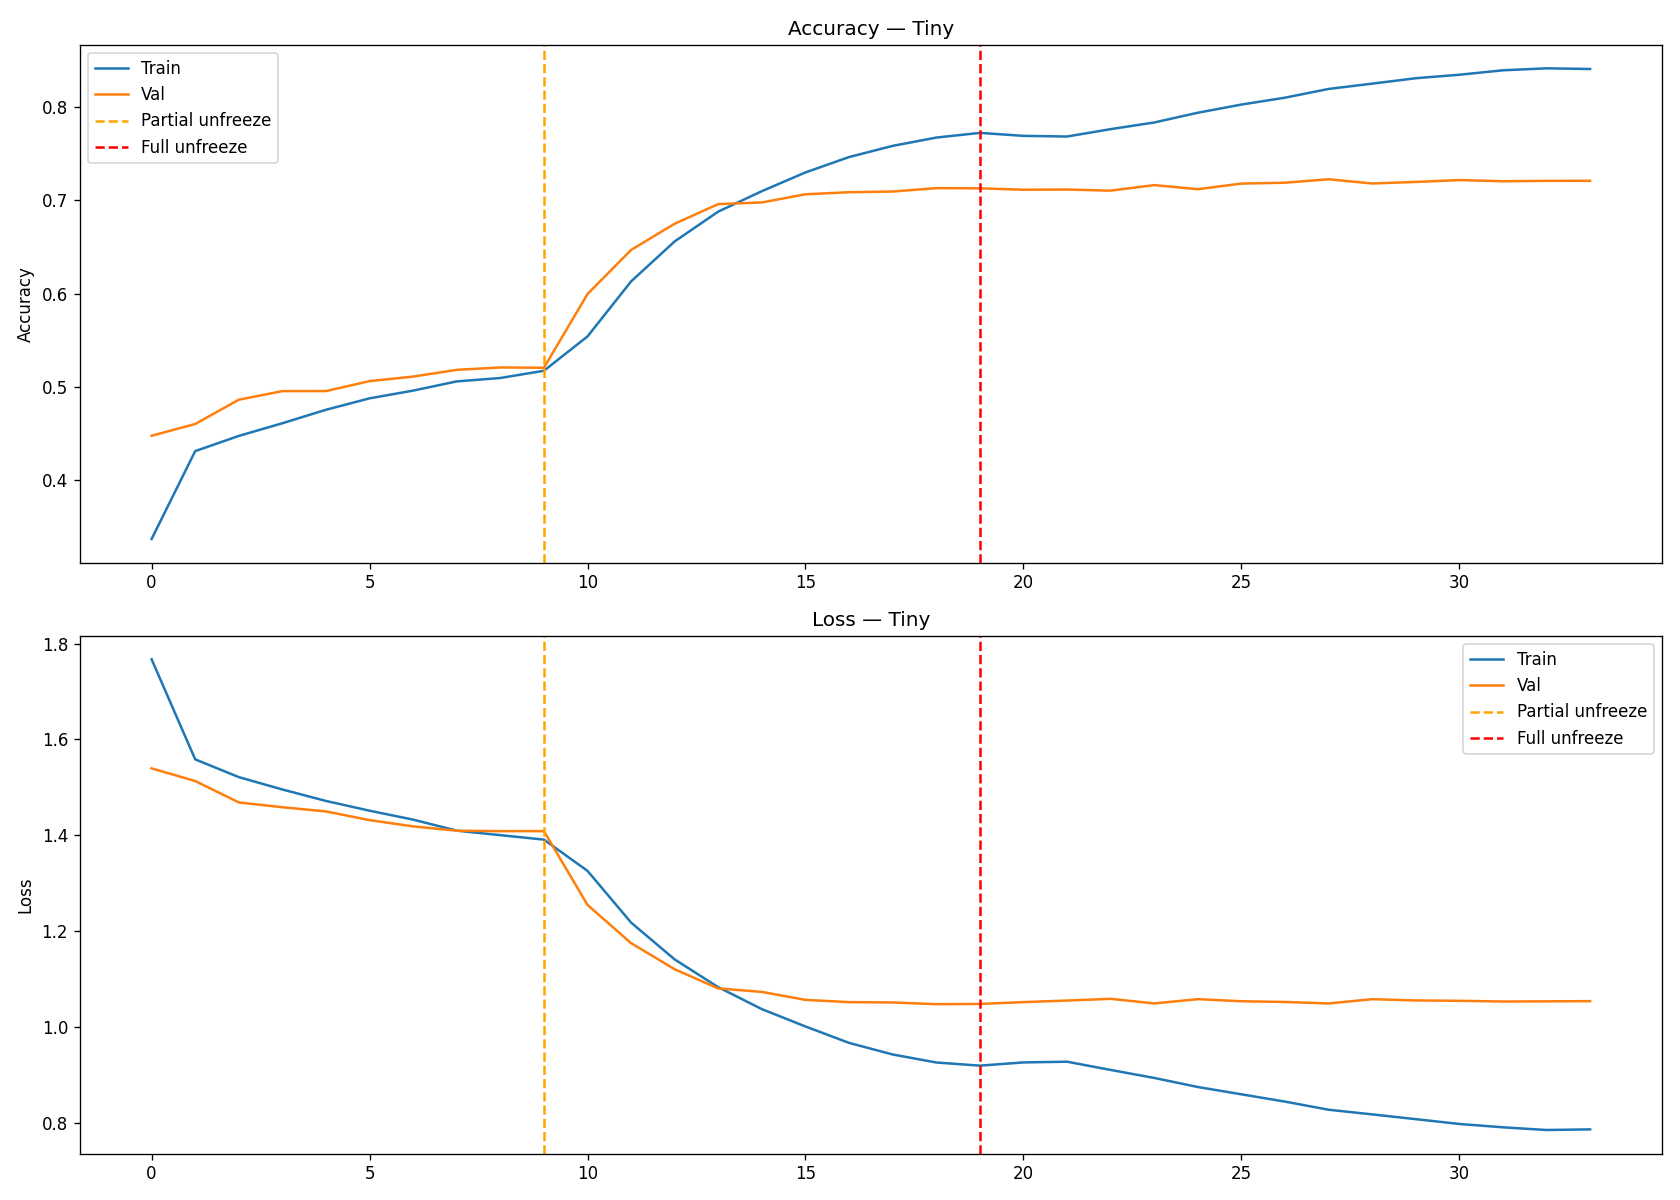
\includegraphics[width=\textwidth]{Tiny_history.png}
        \caption{Tiny - Training History}
        \label{fig:tiny_hist}
    \end{subfigure}
    \hfill
    \begin{subfigure}[b]{0.48\textwidth}
        \centering
        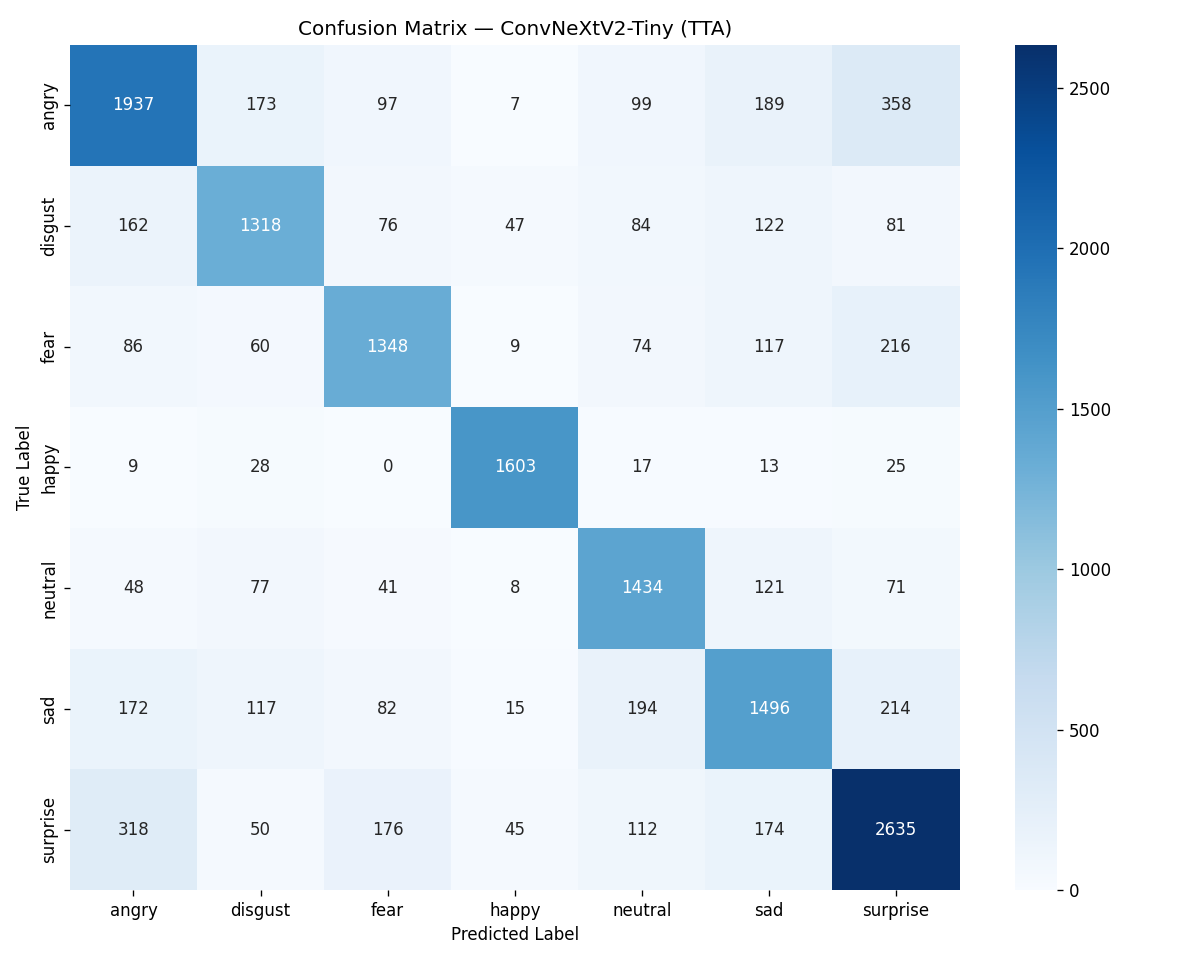
\includegraphics[width=\textwidth]{Tiny_cm.png}
        \caption{Tiny - Confusion Matrix}
        \label{fig:tiny_cm}
    \end{subfigure}
    
    \caption{Comparison of training histories and confusion matrices for the ConvNeXtV2 Atto and Pico models.}
    \label{fig:atto_pico_grid}
\end{figure}

\section{Final Comparison and Benchmarking}
The following table provides a comprehensive summary of the performance metrics achieved by all evaluated architectures. The models are ranked by their validation accuracy. This comparison highlights the transition from custom baseline models to state-of-the-art architectures using advanced fine-tuning techniques on the unified 121,133 image dataset.

\begin{table}[H]
    \centering
    \begin{tabular}{|l|c|c|}
        \hline
        \textbf{Model} & \textbf{Accuracy} & \textbf{Macro-Precision} \\
        \hline
        \textbf{ResNet101 (Fine-tuned, Two-stage)} & \textbf{77.28\%} & \textbf{76.00\%} \\
        \textbf{ResNet50 (Fine-tuned, Two-stage)} & \textbf{75.22\%} & \textbf{73.36\%} \\
        ConvNeXt Tiny (Run 1 - 15 epochs) & 74.56\% & 73.55\% \\
        ConvNeXt Tiny (Run 2 - 10 epochs) & 73.60\% & 72.64\% \\
        second\_model (Custom) & 71.04\% & 70.19\% \\
        VGG19 & 70.07\% & 69.47\% \\
        VGG16 & 68.24\% & 66.57\% \\
        ResNet50 (Initial Training Run) & 67.89\% & 66.21\% \\
        third\_model (Custom) & 67.81\% & 66.42\% \\
        ResNet101 (Initial Training Run) & 67.45\% & 65.88\% \\
        ConvNeXtV2 Huge & 65.60\% & 62.36\% \\
        Xception (with Class Balancing) & 64.92\% & 63.81\% \\
        InceptionV3 (with Class Balancing) & 63.74\% & 62.19\% \\
        ConvNeXtV2 Base & 63.00\% & 59.69\% \\
        ConvNeXtV2 Tiny & 59.70\% & 56.35\% \\
        first\_model (Custom) & 56.17\% & 54.03\% \\
        ConvNeXtV2 Atto & 51.70\% & 48.41\% \\
        ConvNeXtV2 Pico & 40.50\% & 41.97\% \\
        ConvNeXtV2 Tiny & 73.78\% & 74.45\% \\
        \hline
    \end{tabular}
    \caption{Final comparison of model performance metrics on the unified RGB dataset.}
    \label{tab:final_results_updated}
\end{table}

\subsection{Performance Summary}
Analysis of the final benchmarks reveals that the optimized \textbf{ResNet101} and \textbf{ResNet50} architectures, trained using the two-stage fine-tuning approach, have become the superior choices for the vision module. Both models successfully exceeded the project's target accuracy of 75\%, with \textbf{ResNet101} reaching a peak of \textbf{77.28\%} and \textbf{ResNet50} achieving \textbf{75.22\%}. 

While the \textbf{ConvNeXt Tiny} architecture remained a very strong and modern contender (74.56\%), the additional depth and refined training process of the ResNet family allowed for more precise feature extraction in the facial expression domain. The results also show that while custom models like \texttt{second\_model} perform well for their size, they cannot match the generalization capabilities of deeper, fine-tuned residual networks. The application of class weights in other models like Xception provided better balance for minority classes, but the overall accuracy and reliability of ResNet101 make it the definitive leader of this comparison.

\section{Conclusion}
The development of the vision module successfully exceeded its initial goals. Through systematic experimentation and the implementation of an advanced two-stage training strategy, the \textbf{ResNet101} architecture was selected as the primary vision engine, providing the most reliable results with an accuracy of \textbf{77.28\%}. 

The model demonstrates strong generalization and effectively handles the difficult task of distinguishing subtle emotional cues, even in historically problematic pairs like "sad" vs "neutral". This high level of performance ensures that the humanoid head can interact with users in a more natural and responsive manner. Future work will now focus on the deployment phase, specifically optimizing and quantizing the ResNet101 model for real-time inference on the Raspberry Pi platform.

\end{document}